\documentclass{article}

%------------------------------------------------------------------------
% package imports
\usepackage{grffile}
\usepackage{parskip}
\usepackage{graphicx}
\usepackage{float}
\usepackage{caption}
\usepackage{titling}

%\pretitle{Vilniaus Universitetas\\Matematikos ir Informatikos Fakultetas\\Informatikos Institutas\\Programų sistemų studijų programa}
\title{ Laboratorinis darbas \\„Maisto prekių pirkimo asistentas“}
\date{2024-10-06}
\author{Karolis Stoškus\\Evgenij Shapovalov\\Daniil Švager\\Vytenis Narmontas}

% padaro paragraph numeruojamus nuo sectionu
\usepackage{titlesec}
\setcounter{secnumdepth}{4}

%\caption[figure]{labelformat=parens, labelsep=space, name=Pav}
\usepackage{caption}

\captionsetup{
    labelsep=period,
}
\usepackage[figurename=pav]{caption}

\titleformat{\paragraph}
{\normalfont\normalsize\bfseries}{\theparagraph}{1em}{}
\titlespacing*{\paragraph}
{0pt}{3.25ex plus 1ex minus .2ex}{1.5ex plus .2ex}

\setcounter{tocdepth}{4}

% new commands and renewed commands are placed below
\newcommand{\paratoc}[1]{%
\addtocontents{toc}{\protect\contentsline{paragraph}{#1}{\thepage}{\par}}%
}
\renewcommand{\contentsname}{Turinys} % Modifies the name of the table of contents
%------------------------------------------------------------------------
\begin{document}

\maketitle
\vfill
{\large{Vilniaus Universitetas\\Matematikos ir Informatikos Fakultetas\\Informatikos Institutas\\Programų sistemų studijų programa}}
	\pagebreak
	
% Turinys
\tableofcontents
	\pagebreak

% Ivadas
\section{Įvadas}
% Projekto pavadinimai
\subsection{Projekto pavadinimai}
	Pilnas - „Maisto prekių pirkimo asistentas“\\
	Sutrumpintas - „Asistentas“
% Projekto Problemine sritis
\subsection{Projekto Probleminė sritis}
	Parduotuvių lankytojai, apsiperkantys įvairiose maisto prekių parduotuvėse susiduria su kainos, patogumo ir laiko taupymo problemomis. Didžiausia problema įžvelgiama, kai pirkėjams tenka aplankyti nemažą skaičių įvairių parduotuvių, kad rasti specifines prekes, kurių galbūt nėra visose pardavimo vietose. Siekiant padaryti tai kuo greičiau ar pigiau, pirkėjai susiduria su tikru iššūkiu.\\\\
	Problema išryškėja,  kai pirkėjai turi rankiniu būdu dėlioti savo maršrutus ir planuoti  pirkinių sąrašus. Pirkėjui tenka planuoti kelių taškų kelionę, atsižvelgiant į poreikį skirti tam tikrą laiką kiekvienoje parduotuvėje. Norint optimizuoti šį procesą reikia žinoti maršrutus, eismo sąlygas, kuro kainą, parduotuvių darbo laikus, prekių asortimentą bei visu prekių kainas. Kartu tai tampa sunkia užduotimi, kas lemia neefektyvias ar neekologiškas keliones po parduotuves, pamirštus pirkinius arba perteklines išlaidas. Apsipirkti racionaliai tampa dar sunkiau, kai tam tikrus produktus reikia pirkti iš konkrečių parduotuvių, kas dar labiau apsunkina maršruto planavimą.\\\\
	Ši problema išlieka aktuali, nes nėra sprendimo, kuris padėtų vartotojams optimizuoti apsipirkimo kelionę pagal jų pageidavimus, pvz. pasirinkti pigiausią, greičiausią ar ekologiškiausią būdą. Be patogaus įrankio pirkėjai švaisto laiką, pinigus bei nesilaiko numatyto plano lankydamiesi keliose parduotuvėse.
	\pagebreak

% Naudotoju poreikiu analize
\section{Naudotojų poreikių analizė}
\subsection{Suinteresuotų šalių lūkesčiai}
% Pirminiai vartotojai
\subsection*{Pirminiai vartotojai}
\subsubsection*{Pirkėjai}
	Aplikacijos vartotojai naudojasi sistema apsipirkimo tikslams. Sistema leidžia pirkėjams apsipirkinėti greičiau, pigiau ir ekologiškiau negu be jos.
% Antriniai vartotojai
\subsection*{Antriniai vartotojai}
\subsubsection*{Parduotuvės}
	Parduotuvės pastoviai atnaujina parduotuvių sandėlių informaciją, pateikiamą sistemai. Mažmeninės prekybos verslams svarbu, kad jų asortimentas būtų matomas sistemoje, nes tai padeda pritraukti naujų klientų. Taip jos gali išlikti konkurencingos ir neatsilikti nuo kitų tinklų.
\subsubsection*{Ūkininkai}
	Ūkininkai, gaminantys žemės ūkio produkciją, yra suinteresuoti parduoti visa prieinama inventorių, kad nepatirtu finansiniu nuostoliu. Sistema ūkininkams padės jų produkcijai būti prieinamai pirkėjams.
\subsubsection*{Viešasis transportas}
	Viešasis transportas reguliariai atnaujina informaciją apie autobusų maršrutus, kurią naudoja sistemos vartotojai kelionių planavimui. Savivaldybė yra suinteresuota pritraukti daugiau keleivių, kurie moka už kelionės bilietus.
\subsubsection*{Pavėžėjimo paslaugų įmonės}
	Pavėžėjimo paslaugų įmonės siūlo automobilių trumpalaikę nuomą arba pavėžėjimo paslaugas aplikacijos vartotojams, sistemai parenkant geriausią transportą. Įmonės suinteresuotos pritraukti daugiau klientų, kurie moka už kelionės arba automobilių nuomą.
\subsubsection*{Prekybos tinklų duomenų mokslininkai}
	Mažmeninės prekybos verslų duomenų analitikai gali ypač efektyviai rinkti informaciją apie pirkėjų, naudojančių aplikaciją, elgesį.
% Netiesiogines suinteresuotos salys
\subsection*{Netiesioginės suinteresuotos šalys}
\subsubsection*{Verslo savininkai}
	Sistema suteikia galimybę reklamuoti produktus vartotojams. Verslo savininkai gauna pelną iš užsakytų reklamų.
\subsubsection*{Reklamos užsakovai}
	Reklamos užsakovai turi galimybę reklamuoti savo prekes ar paslaugas vartotojams, kurie naudojasi aplikacija. 
% Konkurentai
\subsection*{Konkurentai}
\subsubsection*{Prekių pristatymo paslaugos}
	„UAB Barbora“ taiko pakavimo ir pristatymo mokesčius bei siūlo ribotą prekių asortimentą (prekės yra pasiūlomos tik iš vienos parduotuvės „Maxima LT, UAB“).\par
„Bolt Services LT, UAB“ priklausantis „Bolt Market“ taip pat taiko pakavimo, pristatymo bei krepšelio mokesčius ir nepasiūlo vartotojui plataus prekių asortimento.\par
„Wolt LT, UAB“ priklausantis „Wolt Market“ irgi taiko pakavimo, pristatymo bei krepšelio mokesčius, bei prideda antkainį produktams.
%Kurimo ir prieziuros komanda
\subsection*{Kūrimo ir priežiūros komanda}
	Už kūrimo ir priežiūros procesą būtų atsakinga programuotojų ir kitų IT specialistų komanda.
	\pagebreak

% Pirkeju poreikiu analize
\subsection{Pirkėjų poreikių analizė}
\subsubsection{Dabartiniai vartotojų poreikiai}
% Bandele su karamele
\paragraph{Bandelė su karamele}
	Penkiolikos metų mokinė Justė po pamokų laukia autobuso. Matydama, kad jis atvažiuos po dešimties minučių, mergina nusprendžia nusipirkti bandelę su karamele. Justė turi du pasirinkimus: nusipirkti ją parduotuvėje arba kepyklėlėje. Mergina siekdama sutaupyti pasirenka nubėgti į parduotuvę. Justė parduotuvėje išsiaiškina, kad bandelės su karamele yra išpirktos. Nusivylusi alkana mergina skuba bėgti į stotelę.\par
Problemos: Justė negalėjo patikrinti ar parduotuvėje bus norima prekė, todėl klaidingai nubėgo į ją o ne į kepyklėlę.\par
Galimybės: Sistema galėtų teikti informaciją apie dabar prieinamas prekes.
% Senjorai taupo
\paragraph{Senjorai taupo}
	Pensininkų pora iš Alytaus Jurgis ir Aldona dėl mažos pensijos stengiasi apsipirkinėti kuo taupiau. Šiandien senoliai turi daug laisvo laiko ir yra pasirengę aplankyti kelias parduotuves, kad rasti geriausias kainas. Patikrinus parduotuvių mobiliąsias programėles, jie nustatė, kad “IKI” parduotuvėje jiems reikiamai mėsai yra taikoma 20\% nuolaida. Nuėjus į artimiausią “IKI” senjorai pamatė, kad nukainuotą mėsą jau išpirko, o daugiausiai jiems tinkanti alternatyva kainuoja septynis eurus už kilogramą. Kadangi tai yra gana brangu, pora dar kartą patikrino kitų netoli esančių parduotuvių programėles, tačiau nerado pilno asortimento kainoraščio, o tik ypatingus pasiūlymus. Siekiant išbandyt savo sėkmę senjorai nusprendė visgi aplankyti ir kitas artimas parduotuves, tačiau niekur nerado reikiamos mėsos pigiau ir galiausiai grižo atgal į “IKI”.\par
Problemos: Senjorų pora neturėjo galimybės sužinoti prekės kainų skirtingose parduotuvėse.\par
Galimybės: Sistemos vartotojui iš apsipirkinėjimo būdų pasirinkus “pigiausią”, sistema pati parinktų optimalų maršrutą per parduotuvės.
% Ona iesko ukiu
\paragraph{Ona ieško ūkių}
	Penkiasdešimtmetė miestietė Ona labai stengiasi palaikyti vietinius ūkius ir nori pirkti būtent iš jų. Moteris žino ūkį, kuris parduoda tik vištų kiaušinius ir kitą, kuris parduoda tik agurkus bei pomidorus. Ona internetu bando ieškoti ir kitų ūkių, kurie parduoda likusius produktus, bet jai vis nepavyksta surinkti reikiamo krepšelio. Nusivylusi Ona nusprendžia apsipirkti parduotuvėje.\par
Problemos: Onai yra per daug sudėtinga pačiai suplanuoti savo apsipirkimo maršrutą, jeigu ji nori pirkti prekes tik iš ūkių, kadangi neegzistuoja paslaugos, leidžiančios vienoje vietoje patogiai matyti visus prieinamus ūkius, jų prekes ir kainas.\par
Galimybės: Sistemos vartotojai, ūkiams integravus savo asortimentą į sistemą, galėtų matyti visus produktus iš visų prieinamų ūkių ir dėlioti savo krepšelį vienoje vietoje.
% Arvydas skuba
\paragraph{Arvydas skuba}
	Arvydas gimtadienio proga pakvietė draugus pas save namo. Jam reikia kuo greičiau įsigyti visus reikiamus gurmaniškai vakarienei produktus, tačiau iki šventės pradžios laiko liko labai mažai. Arvydas tiksliai žino kokių produktų jam reikia ir yra pasiruošęs nupirkti juos už bet kokią kainą, tačiau nežino kuriose parduotuvėse pavyks apsipirkti greičiausiai. Patikrinus “Barbora” pristatymo paslaugų prieinamumą jis mato, kad kurjeris važiuos pernelyg ilgai. Galiausiai Arvydas nusprendžia važiuoti į toli esančią “Maxima XXX”, tikėdamasis, kad tikrai suras visus reikiamus produktus. Atvažiavus, Arvydas viską suranda ir skuba namo, tačiau nespėja paruošti vakarienės laiku ir atėjusiems svečiams tenka palaukti.\par
Problemos: Arvydas, negali greitai sužinoti parduotuvių asortimento, todėl galvoja, kad greičiausias apsipirkimo būdas yra nuvažiuoti į didesnę parduotuvę, nors visi reikiami produktai galėjo būti įsigyti keliose arčiau esančiose mažesnėse parduotuvėse.\par
Galimybės: Sistemos vartotojui sudėjus norimas prekes ir iš apsipirkinėjimo būdų pasirinkus “greičiausią”, sistema parinktų tinkamus transporto būdus ir parduotuvių sąrašą.
	\pagebreak

% Zmoniu, veiklu, konteksto ir technologiju charakteristikos
\subsubsection{Žmonių, veiklų, konteksto ir technologijų charakteristikos}
% Zmones
\subsubsection*{Žmonės}
	Sistemos vartotojai yra visi žmones, perkantis maisto produktus ir gebantis naudotis mobiliąja programėle. Į vartotojus patenka beveik visos amžiaus grupes: jauni žmonės (13-30), vidutinio amžiaus žmonės (30-50), brandaus amžiaus žmonės (50-65), vyresnio amžiaus žmonės (65+). 
% Veiklos
\subsubsection*{Veiklos}
		Apsipirkimas parduotuvėje gali būti tiek spontaniškas vienos prekės įsigijimas, tiek apsipirkimas ilgalaikiam periodui.\par
	Spontaniškas kelių ar vienos prekės pirkimas:\par
	Pirkėjas ateina į parduotuvę norėdamas nusipirkti vieną ar kelias prekes beveik kiekvieną dieną. Tokio dažnio veiklą supaprastinanti sistema turi būti minimalistinė ir greitai prieinama sistemos vartotojui. Veiklos trukmė: nuo 5 iki 20 minučių.\par
	Apsipirkimas ilgalaikiam periodui:\par 
	Pirkėjas apsiperka ilgalaikiam periodui retai ir reguliariai: maždaug kartą į savaitę. Tokio dažnio veiklai svarbus naudotojo rėmimas, kad vartotojui būtų lengviau prisiminti kaip naudotis sistema visais veiklos etapais. Veiklos trukmė: nuo 40 iki 180 minučių.
% Kontekstas
\subsubsection*{Kontekstas}
	Fizinė aplinka 1-ame scenarijuje, kai vartotojas patikrina ar prekė yra prieinama parduotuvėje: bet kuri aplinka.\par
	Fizinės aplinkos etapai 2-ame scenarijuje, kai vartotojas planuoja pilną maisto prekių apsipirkimą:\par
	1.	Rami namų aplinka, pastovus apšvietimas, tyla.\\
	2.	Gatvė, nepastovus apšvietimas, triukšmas.\\
	3.	Parduotuvė, pastovus apšvietimas, triukšmas.\par
	Socialinė aplinka: Individuali veikla.
% Technologiju charakteristikos
\subsubsection*{Technologijų charakteristikos}
	Pirkėjų naudojama kompiuterizuota aplinka yra mobilusis telefonas.\par
	\pagebreak

%Poreikiai ir panaudojimo siekiai
\subsubsection{Poreikiai ir panaudojimo siekiai}
	P1. Justė nori matyti ar prekė šiuo metu yra parduotuvėje, kad žinotų ar verta į ją eiti.\par
	P2. Justė nori turėti galimybę pažymėti prekę, kad vėliau gautų pranešimą, kai prekė vėl bus prekyboje, kad nepraleisti galimybės jos įsigyti.\par
	P3. Jurgis ir Aldona nori matyti visų parduotuvių viso esančio asortimento kainas, kad žinotų kurioje parduotuvėje tam tikra prekė šiuo metu yra pigiausia.\par
	P4. Jurgis ir Aldona nori turėti galimybę suplanuoti pigiausią kelionę į parduotuves, kad įsigytų tam tikrus produktus, įskaitant jų kainas ir išlaidas į transportą, tam kad sutaupytų kuo daugiau lėšų.\par
	P5. Ona nori matyti asortimentą, esantį jos pasirinktame ūkyje ar keliuose ūkiuose, kad žinotų, į kuriuos ūkius verta atvykti.\par
	P6. Ona nori turėti galimybę automatiškai matyti geriausią maršrutą per ūkius, kuriuose ji pasirinko prekes, kad nesiblaškyti tarp kelių programėlių.\par
	P7. Arvydas nori turėti galimybę matyti artimiausių parduotuvių, kuriose yra pažymėti produktai, sąrašą, kad gebėtų apsipirkti kuo greičiau.\par
	P8. Arvydas nori matyti greičiausią būdą apvažiuoti visas reikiamas parduotuves, kurias jam rekomendavo programėlę, kad gebėtų apsipirkti kuo greičiau.
	\pagebreak

% Parduotuves
\subsection{Parduotuvės}
% Dabartiniai vartotoju poreikiai
\subsubsection{Dabartiniai vartotojų poreikiai}
\paragraph{Nuošaliai parduotuvei trūksta klientų}
	Šešiasdešimt ketverių metų parduotuvėlės „Prekės Pigiau“ savininkė Janina susiduria su sunkumais pritraukiant naujus klientus. Ji įprastai yra aplankoma tik vietos gyventojų ir Janinos pažįstamų. Ji bandė pritraukti naujus klientus reklamuodamasi socialiniuose tinkluose, tačiau pastangos buvo bevaisės. Dėl mažo srauto ir pardavimų, Janinai neretai tenka išmesti tinkamą vartoti produkciją, todėl ji patiria nuostolių. \par
Problemos: Janina nesėkmingai bando pritraukti naujus klientus naudodama socialinius tinklus kaip reklamos įrankį.\par
Galimybės: sistema leistų savininkei Janinai lengvai patalpinti savo prekių asortimentą ir padaryti jį prieinamu ir matomu dideliam žmonių skaičiui.
% Zmoniu, veiklu kontekstu ir technologiju charakteristikos
\subsubsection{Žmonių, veiklų konteksto ir technologijų charakteristikos}
% Zmones
\subsubsection*{Žmonės}
	Parduotuvių direktoriai, vadovai ir kiti žmonės, atsakingi už parduotuvės plėtrą.
	Tai vidutinio ir brandaus amžiaus žmonės.
% Veiklos
\subsubsection*{Veiklos}
	Prekių įkėlimas, asortimento atnaujinimas:
	Parduotuvės naudoja sistemą, kad joje automatizuotai talpintų informaciją apie prekes: kainą, aprašymą, kiekį. Veiklos trukmė : pastovi.
% Kontekstas	
\subsubsection*{Kontekstas}
	Ofisas, kompiuteriai, ryški šviesa, kabinetai.
% Technologiju charakteristikos
\subsubsection*{Technologijų charakteristikos}
	Janina naudoja savo asmenį kompiuterį, kad prisijungti prie sistemos.
% Poreikiai ir panaudojimo siekiai
\subsubsection{Poreikiai ir panaudojimo siekiai}
	P9. Janina nori pritraukti naujų klientų, kurie apsipirktų jos parduotuvėlėje „Prekės Pigiau“, kad padidintų pajamas.
	\pagebreak
	
% Ukininkai
\subsection{Ūkininkai}
% Dabartiniai vartotoju poreikiai
\subsubsection{Dabartiniai vartotojų poreikiai}
\paragraph{Ūkininkas plečia verslą}
		Penkiasdešimtmetis ūkininkas Žygimantas iš Tauragės rajono turi savo daržovių ūkį. Jis šiuo metu yra paskelbęs  savo paslaugas „Facebook“ platformoje, tačiau norėtų įkelti savo prekes ir kitose platformose, kad patraukti naujų klientų dėmesį. Iš egzistuojančių svetainių Žygimantas surado „ukyje.lt“, tačiau svetainė pasirodė nepatraukli dėl neužbaigto dizaino ir mažo populiarumo (visoje Lietuvoje daržovių kategorijoje yra tik trys produktai/paslaugos). Kitoje svetainėje „ukiai.lt“, Žygimantas nerado galimybės detaliai išvardyti visų savo siūlomų produktų. Žygimantas, nusivilia esama situacija ir nusprendžia palikti įrašą tik „Facebook“ paskyroje.\par
	Problemos: Žygimantui yra sunku pritraukti naujų klientų internete, dėl tinkamų platformų stokos.\par
	Galimybės: Sistema leistų patogiai paskelbti savoa teikiamas paslaugas ar prekes su kainomis ir detalias aprašymais pirkėjams patogioje aplinkoje.
% Zmoniu, veiklu, konteksto ir technologiju charakteristikos
\subsubsection{Žmonių, veiklų, konteksto ir technologijų charakteristikos}
% Zmones
\subsubsection*{Žmones}
	Vidutinio, brandaus ir vyresnio amžiaus žmonės įsitraukę į ūkinę veiklą bei gebantys naudotis kompiuteriu.
% Veiklos	
\subsubsection*{Veiklos}
	Prekių įkėlimas ir atnaujinimas:\par
	Ūkininkas užeina į sistema, kad įkelti naujus produktus arba atnaujinti esamus, tai yra atnaujinti jų kiekį arba pakeisti aprašymą. Veiklos trukmė: nuo 10 iki 60 minučių.
% Kontekstas	
\subsubsection*{Kontekstas}
	Rami namų aplinka, pastovus apšvietimas, tyla.
% Technologiju	
\subsubsection*{Technologijų}	
	Ūkininkai sistema naudojasi per kompiuterinę „web“ programėlę.
% Poreikiai ir panaudojumo siekiai	
\subsubsection{Poreikiai ir panaudojimo siekiai}
	P11. Žygimantas nori turėti galimybę lengvai ir patogiai matyti ir koreguoti turimą asortimentą ūkyje, kad galėtų pasiekti daugiau pirkėjų ir padidinti pardavimus.
	\pagebreak

% Viesojo transporto poreikiu analize	
\subsection{Viešojo transporto poreikių analizė}
% Dabartiniai vartotoju poreikiai	
\subsubsection{Dabartiniai vartotojų poreikiai}
	\paragraph{Pamirštas viešasis transportas}
		Dėl 2024 metais sutvarkytų kelių ir kuro atpigimo Artūras, finansų ir plėtros direktorius UAB “Vilniaus Viešasis Transportas”, pastebi žmonių, kurie naudojasi autobusų ir troleibusų paslaugomis, kiekio sumenkėjimą, kadangi gyventojai mieliau naudojasi savo automobiliu kelionių po miestą tikslams. Įmonė praranda nemenką dalį biudžeto, kurį būtų galėjusi skirti autobusų atnaujinimui ar vairuotojų atlyginimų didinimui. Norint išspręsti problemą “Vilniaus Viešasis Transportas” ieško būdų reklamuoti savo paslaugas, tačiau reklamų rodomų autobusų televizoriuose neužtenka naujų klientų pritraukimui.\par
	Problemos: UAB “Vilniaus Viešasis Transportas” patiria nuostolį sumažėjus žmonių besinaudojančių paslaugomis kiekiui.\par
	Galimybės: Sistema rekomenduotų vartotojams naudoti viešojo transporto paslaugas, kaip pigų ir greitą būdą kelionėms tarp parduotuvių mieste.
% Zmoniu, veiklu, konteksta ir technologiju charakteristikos	
\subsubsection{Žmonių, veiklų, konteksto ir technologijų charakteristikos}
% Zmones	
\subsubsection*{Žmones}
	Vidutinio amžiaus žmonės dirbantys UAB “Vilniaus Viešasis Transportas”
% Veiklos	
\subsubsection*{Veiklos}
	Transporto priemonių tvarkaraščių įkėlimas ir atnaujinimas:\par
	Prijungta duomenų bazė automatiškai įkelia duomenis į sistemą apie dabartinę autobusų lokaciją ir tvarkaraščius. 
% Kontekstas	
\subsubsection*{Kontekstas}
	Rami namų aplinka, pastovus apšvietimas, tyla.
% Technologiju charakteristika
\subsubsection*{Technologijų charakteristika}	
	Ūkininkai sistema naudojasi per kompiuterinę „web“ programėlę.
% Poreikiai ir panaudojimo siekiai	
\subsubsection{Poreikiai ir panaudojimo siekiai}
	P12 UAB “Vilniaus viešasis transportas” nori, kad sistema primintų potencialiems keleiviams apie viešojo transporto alternatyvą, kad pritrauktų naujus klientus.
	\pagebreak

% Pavezejimo paslaugu imoniu poreikiu analize	
\subsection{Pavežėjimo paslaugų įmonių poreikių analizė}
% Dabartiniai vartotoju poreikiai	
\subsubsection{Dabartiniai vartotojų poreikiai}
	Penkiasdešimtmetis Andrius yra įmonės “AndriausTaxi” savininkas. Dėl naujų konkurentų pavėžėjimo paslaugų rinkoje atsiradimo Andriaus įmonė nukenčia. Kitos įmonės užima didžiulę rinkos dalį, tad savininkas ieško būdų skatinti savo įmonės paslaugų vartojimą. Deja Andriaus įmonė neturi pakankamai didelio biudžeto gerai reklamai, o padarytos akcijos kelionėms nenuvilioja geriau žinomų kompanijų, kaip “Bolt” ir “E-Taxi” vartotojų.\par
	Problemos: Dėl mažo žinomumo rinkoje, Andriui sunkiai sekasi pritraukti naujų klientų. \par
	Galimybės: Patogus įmonės paslaugų prieinamumas sistemoje leistų pirkėjams pastebėti Andriaus paslaugas ir padėtų įmonei surasti naujų klientų.
% Zmoniu, veiklu, konteksta ir technologiju charakteristikos	
\subsubsection{Žmonių, veiklų, konteksto ir technologijų charakteristikos}
% Zmones	
\subsubsection*{Žmones}
	Vidutinio, brandaus amžiaus asmenys vadovaujantys pavežėjimo paslaugų įmonėms.
% Veiklos	
\subsubsection*{Veiklos}
	Automatiškai suteikiama informacija iš duomenų bazės apie automobilių dabartinę lokaciją ir kelionių kainas. 
% Kontekstas	
\subsubsection*{Kontekstas}
	Ofiso patalpa, daug kompiuterių, balta šviesa.
% Technologiju charakteristika	
\subsubsection*{Technologijų charakteristika}	
	Ūkininkai sistema naudojasi per kompiuterinę „web“ programėlę.
% Poreikiai ir panaudojimo siekiai	
\subsubsection{Poreikiai ir panaudojimo siekiai}
	P12 UAB “Vilniaus viešasis transportas” nori, kad sistema primintų potencialiems keleiviams apie viešojo transporto alternatyvą, kad pritrauktų naujus klientus.
	\pagebreak

% Duomenu mokslininku poreikiu analize
\subsection{Duomenų mokslininkų poreikių analizė}
% Dabartiniai vartotoju poreikiai
\subsubsection*{Dabartiniai vartotoju poreikiai}
	Trisdešimt vienerių Tautvydas yra prekybos tinklo duomenų analitikas. Jis bando išanalizuoti duomenis apie parduotuvės pirkėjus, tačiau turi per mažai duomenų šaltinių. Tautvydas bando rinkti informaciją iš savo parduotuvės kurjerių paslaugų programėles, tačiau didžiausia pirkėjų dalis apsiperka gyvai. Duomenys apie gyvai apsiperkančius žmones yra labai riboti, todėl Tautvydas savo analizėje remiasi tik programėlės vartotojų duomenimis, kas negatyviai paveikia jo darbo rezultatus.\par
Problemos: Tautvydas, norėdamas gauti kuo daugiau duomenų apie savo parduotuvės pirkėjus susiduria su duomenų šaltinių trukumu.\par
Galimybės: Pirkėjams, kurie apsiperka gyvai, pradėjus naudotis sistema, Tautvydui atsirastu be galo daug naujų duomenų šaltinių, pavyzdžiui duomenys apie vartotojų elgesį renkant produktus.
% Zmoniu, veiklu konteksto ir technologiju charakteristikos
\subsubsection{Žmonių, veiklų, konteksto ir technologijų charakteristikos}
% Zmones	
\subsubsection*{Žmones}
	Vidutinio amžiaus žmonės, dirbantys duomenų mokslo srityje.
% Veiklos	
\subsubsection*{Veiklos}
	Parduotuvių prekių, pardavimų ir kitų duomenų gavimas.
% Kontekstas	
\subsubsection*{Kontekstas}
	Ofisas, ryški šviesa, kompiuteris ir monitorių šviesa
% Technologiju charakteristika	
\subsubsection*{Technologijų charakteristika}	
	Darbo kompiuteris, duomenų bazė.
% Poreikiai ir panaudojimo siekiai	
\subsubsection{Poreikiai ir panaudojimo siekiai}
	P15. Duomenų mokslininkai nori gauti kuo daugiau tikslios informacijos iš parduotuvių tinklų, kad galėtų tinkamai atlikti savo darbą.
	\pagebreak

% Ikvepencios dizaino idejos
\subsection{Įkvepiančios dizaino idėjos}
	\centering
	\begin{figure}[H]
		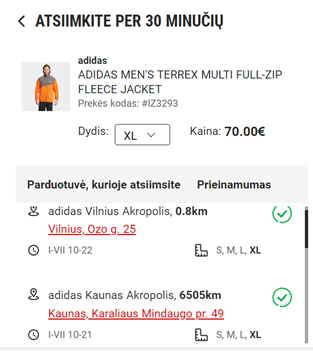
\includegraphics{./images/Picture1.png}
		\caption{Langas, rodantis specifinę informaciją apie prekę ir pasirinkimus susijusius su ta preke (P1, P2)}
		\label{Pav:picture1}
	\end{figure}
	\begin{figure}[H]
		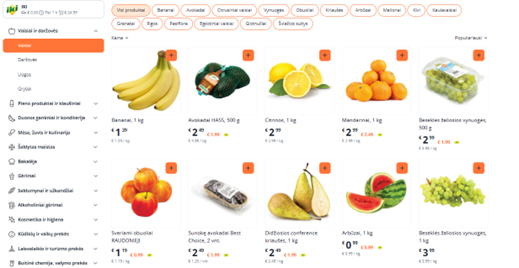
\includegraphics{./images/Picture2.png}
		\caption{Langas, rodantis visas prekes ir jų kainas. Galimas prekių filtravimas pagal lokaciją, paruotuvę, kainą ir kitus pasirinkimus (P3)}
		\label{Pav:picture2}
	\end{figure}
	\begin{figure}[H]
	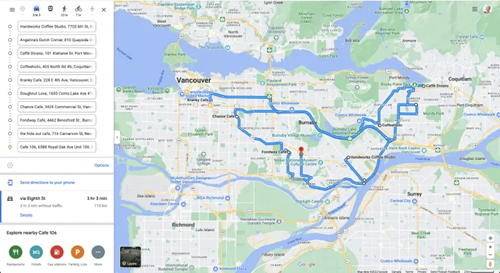
\includegraphics{./images/Picture3.png}
		\caption{Langas, rodantis žemėlapį su informacija apie kelionės laikus ir maršruto pasirinkimus, bei kelionės kainą (P4, P5, P8)}
		\label{Pav:picture3}
	\end{figure}
	\begin{figure}[H]
		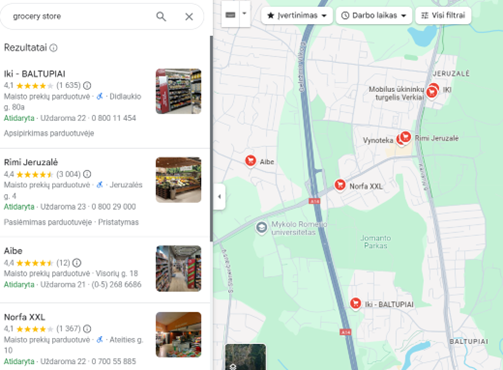
\includegraphics[width=0.75\textwidth]{./images/Picture4.png}
		\caption{Langas rodantis artimiausias parduotuves (P7)}
		\label{Pav:picture4}
	\end{figure}
	\begin{figure}[H]
		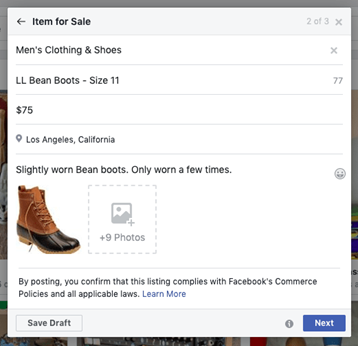
\includegraphics[width=0.75\textwidth]{./images/Picture5.png}
		\caption{Langas, rodantis pasirinkimus norint paskelbti savo parduodamą prekę. Pasirinkimai yra: pavadinimas, kaina, kiekis, nuotraukos ir t.t.(P10, P11)}
		\label{Pav:picture5}
	\end{figure}
\end{document}